\documentclass{article}[18pt]
\usepackage{../../../../format}
\lhead{A Level Maths - S2}
\usepackage{enumitem} %Helps with lists in tables
\setitemize{noitemsep,topsep=-5pt,leftmargin=*}%Compress list

\begin{document}
\begin{center}
\underline{\huge S2 Cheat Sheet}
\end{center}
\section{Binomial and Poisson}
\subsection{Be able to list the assumptions}
\begin{tabularx}{\textwidth}{|X|X|}
\hline
Binomial&Poisson\\
\hline
\begin{itemize}
\item Fixed number of trials
\item Probability of success constant
\item Each trial is independent
\item Each trial has two outcomes
\end{itemize}&
\begin{itemize}
\item Events occur independently
\item No simultaneous events
\item A fixed rate at which events occur
\end{itemize}\\
\hline
\end{tabularx}
\subsection{Geometric distribution questions - Binomial}
Where $X$ is the distribution for the number of successes and Y is the distribution for the number of failures, and n is taken from the distribution
$$P(X<k)=P(Y>n-k)$$
$$P(X\geqslant k)=P(Y\leqslant n-k)$$
\subsection{Finding an unknown n or p from a context}
Set up the probability described in terms of the binomial distribution formula, then solve.\\
\textbf{Example}\\
\textit{I play a game for which the probability of winning is 0.7. If I win every game, what is the smallest number of times I play such that the probability of winning every game is less than 0.01?}\\
$$P(X=n)=0.7^n<0.01$$
$$n\log(0.7)<\log(0.01)$$
$$n>\frac{\log(0.01)}{\log(0.7)}=12.9$$
At least 13 games
\subsection{Solving double inequalities}
\textit{Given $X\sim B(50,0.6)$ find the smallest value of k such that $P(X<k)\geqslant0.9$}
$$X\sim B(50,0.6) \quad Y\sim B(50,0.4)$$
$$P(X<k)=P(Y>50-k)\geqslant0.9$$
$$1-P(Y\leqslant 50-k)\geqslant 0.9$$
$$P(Y\leqslant50-k)\leqslant0.1$$
$$50-k\leqslant15$$
$$k\geqslant35 \therefore k=35$$
\newpage
\subsection{Feeding a poisson into a binomial}
Sometimes the probability calculated by possion can then be fed into binomial for a further calculation, for example:\\
\textit{Defects occur at a rate of 0.5 per 10cm. If bob boys 6 planks each of length 100cm, find the probability fewer than 2 planks contain at most 3 defects}
$$X\sim P_o(5) \quad P(X\leqslant3)=0.2560$$
$$Y\sim B(6,0.256) \quad P(Y<2)=0.4987$$
\section{Continuous random variables}
\subsection{Find the probability of a range of values}
$$P(a<X<b)=\int^b_a f(x) \ dx$$
$$P(X>a)=\int^\infty_a f(x) \ dx$$
For the second term, the probability will become zero after a certain value of x, use this as the upper limit
\subsection{Point probabilities}
The probability at any given value of x for a continuous random variable is zero
\subsection{State the PDF given a graph}
The PDF from a graph is the equations of the lines over the range, but it is important to include the statement that the probability is zero otherwise, for example\\
$
  f(x)=\left\{
  \begin{array}{@{}ll@{}}
    \frac{1}{2}(x-3), & \text{for}\ 3\leq x \leq 5  \\
    0, & \text{otherwise}
  \end{array}\right.
$
\subsection{Calculate measures of location and spread}
Mean and variance and $E(X^2)$ are given on the formula book.\\
To calculate quartiles/deciles set $F(x)$ equal to the location through the distribution and solve. For example the first quartile would be found using $F(x)=0.25$ and the third quartile would be found using $F(x)=0.75$.\\
The mode can be found either graphically or where $f'(x)=0$, making sure that $f''(x)<0$
\subsection{Converting between f(x) and F(x)}
To find $F(x)$, integrate f(x), the +c should be used to make sure that the start of the next range is equal to the previous range
\subsection{Finding greater than probabilities}
As the probability of any given value:
$$P(X\geqslant10)=1-P(X\leqslant10)$$
Unlike for discrete distributions
\newpage
\section{Continuous uniform distribution}
\subsection{Proof of formulas on the data sheet}
\subsubsection{Mean}
$f(x)=\frac{1}{b-a}$
$$E(x)=\frac{1}{b-a}\int_a^bx \ dx=\frac{1}{b-a}\times\frac{1}{2}\Big[x^2\Big]^b_a=\frac{b^2-a^2}{2(b-a)}=\frac{(b-a)(b+a)}{2(b-a)}=\frac{1}{2}(a+b)$$
\subsubsection{Variance}
$f(x)=\frac{1}{b-a}$
$$E(x^2)=\frac{1}{b-a}\int_a^bx^2 \ dx=\frac{1}{b-a}\times\frac{1}{3}\Big[x^3\Big]^b_a=\frac{b^3-a^3}{3(b-a)}=\frac{(b-a)(a^2+ab+b^2)}{3(b-a)}=\frac{a^2+ab+b^2}{3}$$
$$Var(x)=E(x^2)-(E(x))^2$$
$$Var(x)=\frac{a^2+ab+b^2}{3}-\frac{(a+b)^2}{4}=\frac{4a^2+4ab+4b^2}{12}-\frac{3a^2+6ab+3b^2}{12}=\frac{a^2-2ab+b^2}{12}=\frac{(b-a)^2}{12}$$
\subsection{Finding probability over a range}
When finding the probability over a range, multiply the PDF by the width, but remember to check that the range does not extend beyond the range of the distribution, if so, multiply by the width that overlaps with the distribution.
\section{Approximations}
\begin{center}
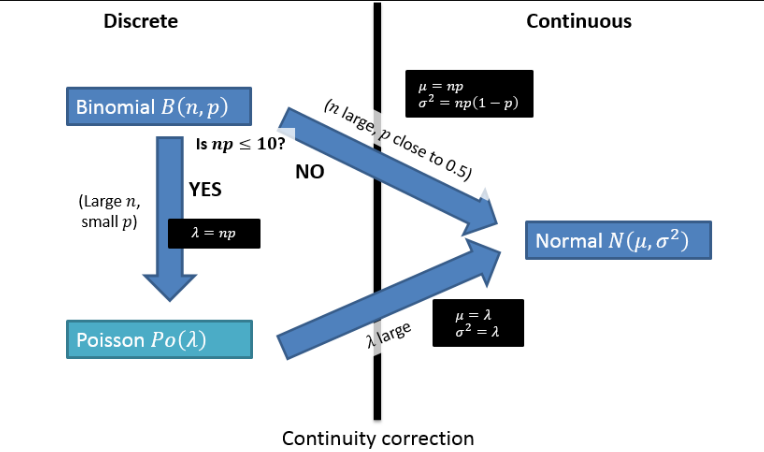
\includegraphics[width=10cm]{approx.png}
\end{center}
All the values for approximation are given on the formula book
\subsection{Continuity correction}
Continuity correction is required when converting from a discrete to a continuous distribution.\\
Method:
\begin{itemize}
\item Make sure the inequality uses $\geqslant$ or $\leqslant$
\item "Extend" the range by 0.5 at each end
\end{itemize}
\newpage
\subsection{Method for a normal approximation}
\begin{enumerate}
\item Determine the correct approximation to use
\item Identify the original distribution
\item Write the approximation
\item Carry out continuity correction
\item Find the probability
\end{enumerate}
\section{Population and samples}
\subsection{Definitions}
\begin{itemize}
\item \textbf{Statistic} - A random variable which is some function of the sample and not dependent on any population parameters
\item \textbf{Population} - A collection of all items
\item \textbf{Sample} - Some subset of the population which is intended to be representative of the population
\item \textbf{Census} - When the entire population is samples
\item \textbf{Sampling unit} - Individual member or element of the population or sampling frame
\item \textbf{Sampling frame} - A list of all sampling units or all the population
\item \textbf{Sampling distribution} - All possible samples that are chosen from a population, the values of a statistic and the associated probabilities.
\end{itemize}

\end{document}